\section{Algorithmes}
Dans ce chapitre nous expliquerons le fonctionnement des algorithmes
du RST en commençant par leur speudocode puis par leur
implémentation. Nous parlerons par la suite d'une heuristique, le
\quickreduct

\subsection{Pseudocode}
Concernant les algortihmes du RST, nous les avons nommé ainsi :
\begin{itemize}
	\item IND et IND\_C
	\item b\_lower et b\_upper
	\item POS\_C et NEG\_C
\end{itemize}
Pour décrire les algorithmes nous utiliserons la notation suivante : \\
(numéro de ligne) : explication. \\
Commençons par IND et IND\_C.
\subsubsection{\ind}
Les deux algorithmes sont similaires, IND regroupe les objets possèdants
les mêmes valeurs pour les C attributs, alors que IND\_C regroupe
les objets possèdants les mêmes valeurs pour tous les attributs.
\begin{algorithm}[h!]
	\SetAlgoLined
	\LinesNumbered
	\SetKwInOut{Input}{Input}
	\Input{DS : Le système de décision \\
		C : La liste des attributs \\
		d :  le nom de la colonne de décision.
	}
	\KwResult{IND : La liste des identifiants identiques}
	$ind \gets \{\}$ \;
	$IS \gets DS.drop(d)$ \;
	$groupe \gets IS.groupby(C)$ \;
	\For{groupe in groupes}{
		$ind.append(g[index])$ \;
	}
	\caption{Algorithme IND}
\end{algorithm}

\begin{algorithm}[h!]
	\SetAlgoLined
	\LinesNumbered
	\SetKwInOut{Input}{Input}
	\Input{DS : Le système de décision \\
		d :  le nom de la colonne de décision.
	}
	\KwResult{IND\_C : La liste des identifiants identiques}
	$ind\_c \gets \{\}$ \;
	$IS \gets DS.drop(d)$ \;
	$groupe \gets IS.groupby(IS.columns)$ \;
	\For{groupe in groupes}{
		$ind\_c.append(g[index])$ \;
	}
	\caption{Algorithme IND\_C}
\end{algorithm}
\newpage
Le fonctionnement des algorithmes est le suivant : \\
(1) : Nous déclarons un ensemble vide. Cet ensemble contiendra des
sous-ensembles d'index d'objets possédant les mêmes caractéristiques. \\
(2) : Nous gardons uniquement le système d'information
en supprimant la colonne décision. \\
(3) : Nous regroupons les objets en fonction d'une sous-ensemble
d'attributs C ou en fonction de tous les attributs IS.colonne.
Cela nous donne une liste de tuple composé de deux éléments. Le premier
est un ensemble d'attributs, et le deuxième est un ensemble d'objets possédant
les mêmes valeurs pour cet ensemble d'attributs. \\
(4) : Pour chaque groupe, nous ajoutons dans l'ensemble initial
l'ensemble des des objets en gardant uniquement leurs index. \\
Passons maintenant à la fonction calculant la \bupper.
\subsubsection{\bupper, \blower et \bboundary}
\begin{algorithm}[h!]
	\SetAlgoLined
	\LinesNumbered
	\SetKwInOut{Input}{Input}
	\Input{DS : Le système de décision. \\
		ind\_c : La liste des objets indiscernables. \\
		d :  le nom de la colonne de décision. \\
		d\_value : la valeur de décision.
	}
	\KwResult{Cxi : la \blower}
	$X \gets DS.groupby(d)$\;
	$Xi \gets X[d\_value]$\;
	\For{$index \gets Xi.index$}{
		$idc\_obj \gets groupe\_ind\_c\_obj(index)$ \;
		$possede\_indiscernable \gets Faux$ \;
		\If{$len(idc\_obj) \neq 0$}{
			\For{index\_obj2 in idc\_obj}{
				\If{$DS[index][d] != DS[index\_obj2][d]$}{
					$possede\_indiscernable \gets Vrai$
				}
			}
		}
		\If{$possede\_indiscernable == Faux$}{
			$CXi.append(index)$
		}
	}
	\caption{Algorithme $b\_lower$}
\end{algorithm}
Pour cet algorithme nous commençons par grouper les objets en fonction de
leur valeurs de décision d. Nous aurons donc pour chaque valeur de d un
groupe avec x indices d'objets. Puis nous gardons le groupe correspondant
à la valeur de $d\_value$. Pour chaque index d'objet o nous l'ajoutons dans
CXi sauf s'il est dans un groupe indiscernable avec un autre objet o'
tel que $d(o) \neq d(o')$. \\
\newpage
Expliquons le fonctionnement de l'algorithme : \\
(1) : Nous regroupons les objets du système de décision en fonction
de leurs valeurs de décision. \\
(2) : Nous gardons uniquement le groupe dont la valeur est égal à
$d\_value$. \\
(3) : Nous parcourons les indexes des objets de chaque groupes. \\
(4) : groupe\_ind\_c\_obj est une fonction qui renvoie le
groupe indiscernable où se situe l'objet obj en le supprimant du groupe.
Ainsi si il est seul dans le groupe, la liste
renvoyé sera vide, sinon nous aurons la liste des objets indiscernables. \\
(6) :  Si l'objet n'est pas seul dans son groupe. \\
(7) : Nous parcourons les objets indiscernables. \\
(8) : Si un des objets indiscernable possède une valeur de décision
différente, nous ne devons pas les ajouter dans CXi. \\
Nous avons un algorithme similaire pour calculer la \blower. \\
\begin{algorithm}[h!]
	\SetAlgoLined
	\LinesNumbered
	\SetKwInOut{Input}{Input}
	\Input{DS : Le système de décision. \\
		ind\_c : La liste des objets indiscernables. \\
		d :  le nom de la colonne de décision. \\
		d\_value : la valeur de décision.
	}
	\KwResult{Cxi : la \blower}
	$X \gets DS.groupby(d)$\;
	$Xi \gets X[d\_value]$\;
	\For{$index \gets Xi.index$}{
		$idc\_obj \gets groupe\_ind\_c\_obj(index)$ \;
		$possede\_indiscernable \gets Faux$ \;
		$sous\_liste \gets \{\}$ \;
		\If{$len(idc\_obj) \neq 0$}{
			\For{index\_obj2 in idc\_obj}{
				\If{$DS[index][d] != DS[index\_obj2][d]$}{
					$sous\_liste.append(index\_obj2)$
				}
			}
		}
		$CXi.concat(sous\_liste)$
	}
	\caption{Algorithme $b\_lower$}
\end{algorithm} \\
La différence entre ces deux algorithmes ce trouve lignes 6, 10, 14 où
nous créons une liste contenant un objet ainsi que tous ces objets
indiscernables que nous ajoutons à CXi. \\
\newpage
Avec ces deux algorithmes, nous pouvons calculer la \bboundary. \\
\begin{algorithm}[h!]
	\SetAlgoLined
	\LinesNumbered
	\SetKwInOut{Input}{Input}
	\Input{DS : Le système de décision. \\
		bupper : La \bupper. \\
		blower : La \blower.
	}
	\KwResult{$BX_C$ : La \bboundary}
	$BX_C \gets bupper - blower$ \;
	\caption{Algorithme $b\_boundary$}
\end{algorithm} \\
Nous passons aux fonctions \posreg et \negreg.
\subsubsection{\posreg et \negreg}
\begin{algorithm}[h!]
	\SetAlgoLined
	\LinesNumbered
	\SetKwInOut{Input}{Input}
	\Input{DS : Le système de décision. \\
		d :  le nom de la colonne de décision.
	}
	\KwResult{$POS_C\{(d)\}$ : La \posreg}
	$d\_values \gets DS[d]$ \;
	$POS_C \gets \{\}$ \;
	$ind\_c \gets IND\_C(DS, d)$ \;
	\For{$d\_value$ in $d\_values$}{
		$POS_C.concat(b\_lower(DS, ind\_c, d, d\_value))$
	}
	\caption{Algorithme $POS\_C$}
\end{algorithm}
Le fonctionnement de l'algorithme est le suivant : \\
(1) : Nous commençons par prendre toutes les décisions (sans doublons)
du système de décision. \\
(4) : Pour chaque valeur de décision nous calculons la \blower et nous
l'ajoutons dans $POS\_C$. \\
Nous avons aussi la version calculant la \posreg pour C attributs. \\
\begin{algorithm}[h!]
	\SetAlgoLined
	\LinesNumbered
	\SetKwInOut{Input}{Input}
	\Input{DS : Le système de décision. \\
		C :  le nom des attributs.
		d :  le nom de la colonne de décision.
	}
	\KwResult{$POS\{(d)\}$ : La \posreg}
	$ds \gets DS[C + d]$ \;
	$ind \gets IND(ds, d, C)$ \;
	$d\_values \gets ds[d]$ \;
	$POS \gets \{\}$ \;
	\For{$d\_value$ in $d\_values$}{
		$POS.concat(b\_lower(ds, ind, d, d\_value))$
	}
	\caption{Algorithme POS}
\end{algorithm}
\newpage
L'algorithme pour la \negreg est presque identique. \\
\begin{algorithm}[h!]
	\SetAlgoLined
	\LinesNumbered
	\SetKwInOut{Input}{Input}
	\Input{DS : Le système de décision. \\
		ind\_c : La liste des objets indiscernables. \\
		d :  le nom de la colonne de décision.
	}
	\KwResult{$NEG_C\{(d)\}$ : La \negreg}
	$d\_values \gets DS[d]$ \;
	$NEG_C \gets \{\}$ \;
	\For{$d\_value$ in $d\_values$}{
		$NEG_C.concat(b\_lower(DS, ind\_c, d, d\_value))$
	}
	$NEG_C \gets diff\_list(DS.index, NEG_C)$
	\caption{Algorithme $NEG\_C$}
\end{algorithm} \\
La différence étant ligne (6), nous faisons la différences entre
l'univers et la \negreg. \\
A l'aide de la \posreg nous pouvons calculer le \reduct et le \core.
\subsubsection{\reduct et \core}
L'algorithme du \reduct est le suivant : \\
\begin{algorithm}[h!]
	\SetAlgoLined
	\LinesNumbered
	\SetKwInOut{Input}{Input}
	\Input{DS : Le système de décision. \\
		d :  le nom de la colonne de décision.
	}
	\KwResult{reducts : Le \reduct}
	$reducts \gets \{\}$ \;
	$POS_C \gets POS\_C(DS, d)$ \;
	$C \gets DS.columns \neq d$ \;
	\For{combi in combinaisons(DS, D)}{
		\If{$combi \neq C$}{
			$pos \gets POS(DS, d, combi)$ \;
			\If{$pos == POS_C$}{
				$reducts.append(combi)$
			}
		}
	}
	\caption{Algorithme reduct}
\end{algorithm} \\
Le détail de cet algorithme est le suivant : \\
(1) : Nous créons un ensemble qui contiendra des sous-ensembles de
\reduct. \\
(2) : Nous calculons la \posreg de l'ensemble des attributs. \\
(3) : Nous prenons l'ensemble des attributs sans la colonne de
décision. \\
(4) : La fonction combinaisons renvoie l'ensemble des combinaisons
possibles d'attributs du DS en paramètres. Nous parcourons donc
chaqu'une des combinaisons. \\
(5) : Si la combinaisons est différente de l'ensemble d'attributs. \\
(6) : Nous calculons la \posreg de la combinaison d'attributs. \\
(7) : Si la \posreg est égal à la \posreg de tous les attributs alors
la combinaison d'attributs est un \reduct. \\
(8) : Nous l'ajoutons dans l'ensemble des \reduct. \\

A l'aide des \reduct nous pouvons calculer le \core. Nous renvoyons
la liste des attributs en communs dans tous les \reduct. \\

Nous avons terminé la partie \rst, nous allons passé à une heuristique
le \quickreduct. \\
\subsubsection{\textit{quickReduct}}
\begin{algorithm}[h!]
	\SetAlgoLined
	\LinesNumbered
	\SetKwInOut{Input}{Input}
	\Input{C : the set of all conditional features \\ D : the set of decision features}
	\KwResult{R : the reduced set of conditional features}
	\SetKwRepeat{Do}{do}{while}
	$R \gets \{\}$ \;
	\Do{$\lambda_R(D) == \lambda_C(D)$}{
		$T \gets R$ \;
		$\forall x \in (C - R)$ \;
		\If{$\lambda_{RU\{x\}}(D) > \lambda_T(D)$}{
			$T \gets R U \{x\}$ \;
		}
		$R \gets T$ \;
	}
	\caption{Algorithme quickReduct}
\end{algorithm}
Explication de l'algorithme : \\
(1) Initialisation d'un ensemble, noté R, vide. Nous stockerons dedans
l'ensemble réduit des attributs. \\
(2) Tant que la dépendance de R n'est pas égal à la dépendance de C. \\
(3) Nous créons un ensemble temporaire, noté T, égal à l'ensemble R. \\
(4) Pour chaque attributs, noté x, présent dans C mais pas dans R. \\
(5) Si la dépendance de R en ajoutant x est supérieur à la dépendance de T. \\
(6) On ajoute x dans l'ensemble T. \\

Ceci terminant les speudocodes, nous allons pouvoir les implémenter.
Avant de parler à proprement parlé de l'implémentation, nous allons
définir l'environnement de travail. \\
Pour implémenter les algorithmes, nous utiliserons :
\begin{itemize}
	\item Un ordinateur portable Dell G5 5587 avec :
	      \begin{itemize}
		      \item Windows 10 Famille.
		      \item 16Go de RAM.
		      \item Intel Core i7-8750 avec une fréquence de 2.20GHz.
	      \end{itemize}
	\item Le logiciel Visual Studio Code pour coder.
	\item L'extension Jupyter v2022.11.1003412109 pour écrire
	      notre notebook.
	\item Nous coderons avec le langage Python.
	\item Anaconda pour gérer l'environnement virtuel, avec un ensemble
	      de bibliothèques comme par exemple \panda et \numpy
	      pour la manipulation d'objets complexes.
	      Mais aussi \textit{sklearn} pour les modèles de machine learning.
\end{itemize}
Nous pouvons à présent parler de l'implémentation des différentes
algorithmes.
\subsection{Implémentation}
Dans cette sous partie nous montrerons l'implémentation des algorithmes.
Comme nous utilisons le Python, nous avons avons du convertir les objets
mathématiques en objet implémenté par le langage Python. Par exemple
les ensembles sont devenus des listes. \\
\subsubsection{\ind}
\begin{lstlisting}
def IND(DS, d, C):
	"""
	Calcule la Indiscernibility Relation pour un attribut.
	
	@param DS le système de décision.
	@param d la décision.
	@param C La liste des attributs.
	
	@return ind la Indiscernibility Relation.
	"""
	ind = []
	IS = DS.drop(d, axis=1)
	group = IS.groupby(C)

	for g in group:
		gDS = pd.DataFrame(g[1])
		ind.append(list(gDS.index))
	ind.sort()
	return ind
\end{lstlisting}
Les paramètres sont DS un \df issue de la bibliothèque \panda. Le
paramètre d, une \str, est le nom de la colonne de décision. Le
dernier paramètre C, une liste de \str,  contenant le nom des
attributs. \\
La fonctionnement de cet algorithme est le suivant : \\
(12) :  La fonction \textbf{drop} est une fonction issue de la
bibliothèque \panda. Nous l'utilisons pour supprimer la
colonne d. \\
(13) : Nous utilisons la fonction \textbf{groupby} pour regrouper les
objets. \\
(15) : Pour chaque groupe d'objets, sous forme de tuple. \\
(16) : Nous convertissons les objets pour utiliser la fonction
\textbf{index}. \\
(17) : Nous ajoutons les tableaux convertis des indexes des objets en
liste. \\
\newpage
\begin{lstlisting}
def IND_C(DS, d):
	"""
	Calcule la Indiscernibility Relation pour tous les
	attributs du système de décision.
	
	@param DS le système de décision.
	@param d la décision.
	
	@return ind_c la Indiscernibility Relation.
	"""
	ind = []
	IS = DS.drop(d, axis=1)
	group = IS.groupby(list(IS.columns))

	for g in group:
		gDS = pd.DataFrame(g[1])
		ind.append(list(gDS.index))
	ind.sort()
	return ind
\end{lstlisting}
L'algorithme fonctionne de la même manière, sauf que nous groupons selon
\textbf{IS.columns}, qui est une fonction de \panda nous renvoyant
la liste des attributs de DS. \\
Passons maintenant à une fonction intermédiaires dont nous avons
parlé durant la partie speudocode.
\begin{lstlisting}
def groupe_ind_c_obj(ind_c, obj):
	"""
	Renvoie le groupe indiscernable de l'objet obj sans ce dernier.

	@param ind_c la liste des objets indiscernable.
	@param obj l'index d'un objet.

	@return le groupe indiscernable de l'objet.
	"""
	for g in ind_c:
		for obj2 in g:
			if obj == obj2:
				copy_g = g.copy()
				copy_g.remove(obj)
				return copy_g
	return []
\end{lstlisting}
L'idée de l'algorithme est la suivante : \\
Pour chaque sous liste dans $ind\_c$, nous parcourons la liste des indexes.
Si nous trouvons l'objet que nous cherchons, nos copions sont groupes
nous le supprimons de son groupe et nous renvoyons son groupe. \\
\newpage
\subsubsection{\blower, \bupper et \bboundary}
\begin{lstlisting}
def b_lower(DS, ind_c, d, d_value):
    """
    Renvoie la B-lower approximation.

    @param DS le système de décision.
    @param ind_c la liste des objets indiscernables.
    @param d le nom de la colonne de décision.
    @param d_value la valeur de décision.

    @return la B-lower approximation.
    """
    X = DS.groupby(d)
    Xi = None
    for name, groupe in X:
        if name == d_value:
            Xi = pd.DataFrame(groupe)

    if Xi is not None:
        CXi = []

        for index in Xi.index:
            # Nous regardons le groupe indiscernable de cet objet.
            idc_obj = groupe_ind_c_obj(ind_c, index)
            
            # Si aucun des objets indiscernables de cet objet n'a une décision différente.
            if not any(DS.at[index_obj2, d] != DS.at[index, d] for index_obj2 in idc_obj):
                CXi.append(index)
        CXi.sort()
        return CXi
    else:
        return "error"
\end{lstlisting}
Le fonctionnement de cet algorithme à été évoqué durant la partie
pseudocode, mais il y a quelques différences. La première étant entre
les lignes (12) et (16) qui permettent de trouver les groupes ou se trouve
la $d\_value$. La deuxième étant les lignes (30) et (31) qui permettent
de selectionner la valeur de décision en fonction de leur indexes.
\newpage
\begin{lstlisting}
def b_upper(DS, ind_c, d, d_value):
    """
    Renvoie la B-upper approximation.

    @param DS le système de décision.
    @param ind_c la liste des objets indiscernables.
    @param d le nom de la colonne de décision.
    @param d_value la valeur de décision.

    @return la B-upper approximation.
    """
    X = DS.groupby(d)
    Xi = None
    for name, groupe in X:
        if name == d_value:
            Xi = pd.DataFrame(groupe)

    if Xi is not None:
        CXi = list(Xi.index)
        for index in Xi.index:
            # Nous regardons le groupe indiscernable de cet objet.
            idc_obj = groupe_ind_c_obj(ind_c, index)
            
            # Si il possède des objets indiscernables.
            list_add = [index_obj2 for index_obj2 in idc_obj
                        if DS.at[index_obj2, d] != DS.at[index, d]]
            CXi += list_add
        CXi.sort()
        return CXi
    else:
        return "error"
\end{lstlisting}
\begin{lstlisting}
def b_boundary(DS, bupper, blower):
	"""
	Calcule la B-boundary region.

	@param DS le système de décision.
	@param bupper la B-upper approximation.
	@param blower la B-lower approximation.

	@return la différence entre les deux approximations.
	"""
	return diff_list(bupper, blower)
\end{lstlisting}
Cette fonction utilise une fonction que nous avons conçu, la fonction
$diff\_list$.
\newpage
\begin{lstlisting}
def diff_list(list1, list2):
	"""
	Renvoie la différence entre deux listes.

	@param list1 une première liste.
	@param list2 une deuxième liste.

	@return les éléments présents dans list1 mais pas dans list2.
	"""
	set_list2 = set(list2)
	diff = [x for x in list1 if x not in set_list2]
	return diff
\end{lstlisting}
Fonction issue du cite \cite{diff_list}.
\subsubsection{\posreg et \negreg}
\begin{lstlisting}
def POS(DS, d, C):
	"""
	Calcul la Positive Region avec les C attributs.

	@param DS Le système de décision.
	@param d La colonne de décision.
	@param C La liste des attributs.

	@return La Positive region des C attributs.
	"""
	attr = C.copy()
	attr.append(d)
	ds = DS[attr]
	ind = IND(ds, d, C)
	d_values = list(ds[d])
	d_values = [*set(d_values)]
	POS = []
	for d_value in d_values:
		POS += b_lower(ds, ind, d, d_value)
	POS.sort()
	return POS
\end{lstlisting}
(11) à (13) : Création d'un \df avec les C attributs qui nous
intéresses.\\
(16) : Permet de supprimer les doublons. \\
(17) à (19) : Nous ajoutons toutes les \blower en fonction de la valeur
de décision $d\_value$. \\
\newpage
\begin{lstlisting}
def POS_C(DS, d):
	"""
	Calcule la Positive Region avec tous les attributs.

	@param DS Le système de décision.
	@param d La colonne de décision.

	@return La Positive region de tous les attributs.
	"""
	d_values = list(DS[d])
	d_values = [*set(d_values)]
	POS_C = []
	ind_c = IND_C(DS, d)
	for d_value in d_values:
		POS_C += b_lower(DS, ind_c, d, d_value)
	POS_C.sort()
	return POS_C
\end{lstlisting}
\begin{lstlisting}
def NEG_C(DS, d):
	"""
	Calcule la Negative Region avec tous les attributs.

	@param DS Le système de décision.
	@param d La colonne de décision.

	@return La Negative region de tous les attributs.
	"""
	d_values = list(DS[d])
	d_values = [*set(d_values)]
	NEG_C = []
	ind_c = IND_C(DS, d)
	for d_value in d_values:
		NEG_C += b_upper(DS, ind_c, d, d_value)
	NEG_C = [*set(NEG_C)]
	neg = diff_list(list(DS.index), NEG_C)
	neg.sort()
	return neg
\end{lstlisting}
(7) : Nous supprimons les doublons. \\
(8) : Nous appliquons la formule donnée dans le chapitre 1. \\
\newpage
\subsubsection{\reduct et \core}
\begin{lstlisting}
def reduct(DS, d):
	"""
	Renvoie toutes les réductions d'attributs possibles.

	@param DS Le système de décision.
	@param d La colonne de décision.

	@return reducts : La liste des réductions.
	"""
	reducts = []
	pos_c = POS_C(DS, d)
	C = list(DS.columns)
	C.remove(d)
	for combi in combinaisons(DS, d):
		liste_combi = list(combi)
		if liste_combi != C:
			pos = POS(DS, d, liste_combi)
			if pos == pos_c:
				reducts.append(liste_combi)
	reducts.sort()

	# minimal set
	min_len = min([len(x) for x in reducts])
	reducts = [x for x in reducts if len(x) == min_len]

	return reducts
\end{lstlisting}
\begin{lstlisting}
def core(reducts):
    """
	Calcul l'intersection de toutes les réductions.

	@param reducts la liste des réductions.

	@return le core du système de décision.
	"""
	return list(reduce(lambda i, j: i & j, (set(x) for x in reducts)))
\end{lstlisting}
Fonction issue du cite \cite{intersection_list}.
\newpage
\subsubsection{\quickreduct}
\begin{lstlisting}
def dependance_attributs(DS, C, d):
    """
	Calcul la dépendance des attributs.

	@param DS Le système de décision.
	@param C la liste des attributs.
	@param d la colonne de décision.

	@return la dépendance des attributs.
	"""
	ds = DS[C]
	if len(list(ds.columns)) == 1 and list(ds.columns)[0] == d:
		return 0
	ind = IND_C(ds, d)
	pos_c = POS_C(ds, ind, d)
	dep = Fraction(len(pos_c), len(ds.index))
	return dep
\end{lstlisting}
\begin{lstlisting}
def quickReduct(DS, d):
    """
	L'algorithme de quickReduct.

	@param DS Le système de décision.
	@param d la colonne de décision.

	@return une sous liste d'attributs.
	"""
	C = list(DS.columns)
	C.remove(d)
	print("C :", C)
	# calcul de lambda C.
	dep_C = my_lambda(DS, DS.columns, d)
	print("dep_C :", dep_C)
	R = []
	while True:
		T = R
		# calcul de lambda T.
		attr = T.copy() + [d]
		dep_T = my_lambda(DS, attr, d)
		print("lambda({}) = {}".format(attr[:-1], dep_T))
		
		# calcul de C - R.
		Rset = set(R)
		C_R = [x for x in C if x not in Rset]
		
		# parcours des attributs.
		for x in C_R:
			# calcul de lambda RU{x}.
			attr2 = R.copy() + [x, d]
			dep_RUx = my_lambda(DS, attr2, d)
			print("lambda({}) = {}".format(attr2[:-1], dep_RUx))
			
			# changement meilleur dépendance.
			if dep_RUx > dep_T:
				T = R.copy() + [x]
				print("changement R =", T)
				attr3 = T.copy() + [d]
				dep_T = my_lambda(DS, attr3, d)
		
		R = T.copy()
		# calcul de lambda R.
		attr4 = R.copy() + [d]
		dep_R = my_lambda(DS, attr4, d)
		print("lambda({}) = {}".format(attr4[:-1], dep_R))
		if dep_R == dep_C:
			break
	return R
\end{lstlisting}
\subsection{Test}
Passons maintenant aux tests. Pour cela nous devons créer des jeux de
tests. Voici un exemple que nous utiliserons pour les algorithmes
issues du \rst : \\
\begin{figure}[h!]
	\centering
	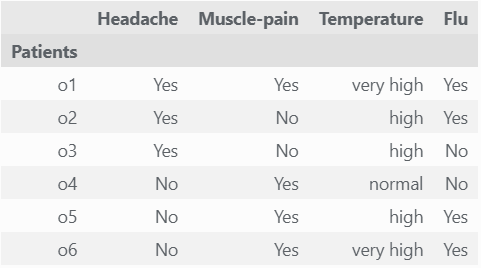
\includegraphics[scale=0.8]{img/df_exemple_1.PNG}
	\caption{Dataframe "df"}
	\label{fig:df_exemple_1}
\end{figure}
\subsubsection{\ind}
Commençons par calculer IND. \\
Si nous prenons uniquement la colonne \headache, nous voyons
les objets $o_1$, $o_2$ et $o_3$ ont la même valeur, "Yes", et les
$o_4$, $o_5$ et $o_6$ ont la même valeur, "No". Nous avons donc le
résultat suivant : \\
$IND_{\{Headache\}} = \{\{o_1, o_2, o_3\}, \{o_4, o_5, o_6\}\}$ \\
Mais si nous prenons les colonnes \headache et
\musclepain, nous voyons que l'objet est le seul à possèdé le
couple de valeur ("Yes", "Yes"), les objets $o_2$ et $o_3$ possèdent
le couple de valeur ("Yes", "No"), enfin les objets $o_4$, $o_5$ et
$o_6$ possèdent le couple de valeur ("No", "Yes"). Nous avons donc le
résultat suivant : \\
$IND_{\{Headache, Muscle-pain\}} = \{\{o_1\} \{o_2, o_3\}, \{o_4, o_5,
	o_6\}\}$ \\
\begin{lstlisting}
ind = IND(df, "Flu", ["Headache"])
ind
Python> [['o1', 'o2', 'o3'], ['o4', 'o5', 'o6']]
ind2 = IND(df, "Flu", ["Headache", "Muscle-pain"])
ind2
Python> [['o1'], ['o2', 'o3'], ['o4', 'o5', 'o6']]
\end{lstlisting}
Nous notons la sortie des cellules Jupiter à la suite de "Python>". \\
Calculons maintenant $IND_C$. \\
Dans le premier exemple nous voyons que $o_1$, $o_4$, $o_5$, et
$o_6$ ne sont identiques à aucun objets et que $o_2$ et $o_3$
sont identiques entre eux. Nous devons obtenir l'ensemble suivant :
$IND_C = \{\{o_1\}, \{o_2, o_3\}, \{o_4\}, \{o_5\}, \{o_6\}\}$. \\
Dans le deuxième exemple nous voyons que $x_1$, $x_4$, $x_5$ et $x_7$
ne sont identiques à aucun autres objets, $x_2$ et $x_8$ sont
identiques entre eux et $x_3$ et $x_6$ de même. Nous devons donc
obtenir l'ensemble suivant : \\
$IND_C = \{\{x_1\}, \{x_2, x_8\}, \{x_3, x_6\}, \{x_4\}, \{x_5\},
	\{x_7\}\}$. \\
Avec notre algorithme, nous obtenons les résultats suivants :
\begin{lstlisting}
ind_c1 = IND_C(df, "Flu")
ind_c1
Python> [['o1'], ['o2', 'o3'], ['o4'], ['o5'], ['o6']]
ind_c2 = IND_C(df2, "e")
ind_c2
Python> [['x1'], ['x2', 'x8'], ['x3', 'x6'], ['x4'], 
['x5'], ['x7']]
\end{lstlisting}
\subsubsection{\blower, \bupper et \bboundary}
Nous avons deux valeurs pour la décisions,
"Yes" ou "No". Cela implique que nous avons deux classes
d'équivalences : \\
$X_1 = \{o_j | Flu(o_j) = \{Yes\}\} = \{o_1, o_2, o_5, o_6\}$ et
$X_2 = \{o_j | Flu(o_j) = \{No\}\} = \{o_3, o_4\}$ \\
Si nous calculons les \blower, notées $\underline{C}X_1$ et
$\underline{C}X_2$, nous obtenons les résultats suivants : \\
$\underline{C}X_1 = \{o_1, o_5, o_6\}$ et
$\underline{C}X_2 = \{o_4\}$ \\
Nous enlevons $o_2$ dans $\underline{C}X_1$ car $o_2$ est dans le même
groupe $IND_C$ que $o_3$. Pour la même raison nous supprimons $o_3$
dans l'équation $\underline{C}X_2$. \\
Si nous calculons les \bupper, notées $\Bar{C}X_1$ et
$\Bar{C}X_2$, nous obtenons les résultats suivants : \\
$\Bar{C}X_1 = \{o_1, o_2, o_3, o_5, o_6\}$ et
$\Bar{C}X_2 = \{o_2, o_3, o_4\}$ \\
Enfin nous pouvons calculer les \bboundary. \\
$BN_C(X_1) = \{o_2, o_3\} $ et $BN_C(X_2) = \{o_2, o_3\}$\\
Avons nos algorithmes nous avons les résultats suivants :
\begin{lstlisting}
blower_yes = b_lower(df, ind_c, "Flu", "Yes")
Python> ['o1', 'o5', 'o6']
blower_no = b_lower(df, ind_c, "Flu", "No")
Python> ['o4']

bupper_yes = b_upper(df, ind_c, "Flu", "Yes")
Python> ['o1', 'o2', 'o3', 'o5', 'o6']
bupper_no = b_upper(df, ind_c, "Flu", "No")
Python> ['o2', 'o3', 'o4']

b_boundary(df, bupper_yes, blower_yes)
Python> ['o2', 'o3']
b_boundary(df, bupper_no, blower_no)
Python> ['o2', 'o3']
\end{lstlisting}
$blower\_yes$ correspond à $\underline{C}X_1$, $bupper\_yes$ correspond
à $\Bar{C}X_1$, $blower\_no$ correspond à $\underline{C}X_2$, et
$bupper\_no$ correspond à $\Bar{C}X_2$. \\
\subsubsection{\posreg et \negreg}
Nous avons la \posreg pour un ou plusieurs attributs : \\
$POS_{\{Headache, Muscle-pain\}}(\{d\}) = \{o_1\}$ \\
$POS_{\{Headache, Temperature\}}(\{d\}) = \{o_1, o_4, o_5, o_6\}$ \\
$POS_{\{Muscle-pain, Temperature\}}(\{d\}) = \{o_1, o_4, o_5, o_6\}$ \\
$POS_{\{Headache\}}(\{d\}) = \emptyset $ \\
$POS_{\{Muscle-pain\}}(\{d\}) = \emptyset $ \\
$POS_{\{Temperature\}}(\{d\}) = \{o_1, o_4, o_6\}$ \\
Avec notre algorithmes nous avons le résultat suivants :
\begin{lstlisting}
for combi in combinaisons(df, "Flu"):
liste_combi = list(combi)
print("POS{{{}}} = {}".format(liste_combi, POS(df, "Flu", liste_combi)))
Python> POS{['Headache']} = []
POS{['Muscle-pain']} = []
POS{['Temperature']} = ['o1', 'o4', 'o6']
POS{['Headache', 'Muscle-pain']} = ['o1']
POS{['Headache', 'Temperature']} = ['o1', 'o4', 'o5', 'o6']
POS{['Muscle-pain', 'Temperature']} = ['o1', 'o4', 'o5', 'o6']
POS{['Headache', 'Muscle-pain', 'Temperature']} = ['o1', 'o4', 'o5', 'o6']
\end{lstlisting}
Dans le code ci-dessus, nous calculons la \posreg pour
toutes les combinaisons d'attributs possibles.
Ensuite nous avons la \posreg et \negreg pour tous les
attributs : \\
$POS_C = \underline{C}X_1 \cup \underline{C}X_2
	= \{o_1, o_5, o_6\} \cup \{o_4\}
	= \{o_1, o_5, o_6, o_4\}$ \\
$NEG_C = U - (\Bar{C}X_1 \cup \Bar{C}X_2)
	= \{o_1, o_2, o_3, o_4, o_5, o_6\} - (\{o_1, o_2, o_3,
	o_5, o_6\} \cup \{o_2, o_3, o_4\})
	= \emptyset $ \\
Avec nos algorithmes nous avons les résultats suivants :
\begin{lstlisting}
POS_C(df, "Flu")
Python> ['o1', 'o4', 'o5', 'o6']
NEG_C(df, "Flu")
Python> []
\end{lstlisting}
\subsubsection{\reduct et \core}
Si nous reprenons les calculs des \posreg pour chaque
attributs, nous voyons que les \reduct sont : \\
$\{Headache, Temperature\}$ et $\{Muscle-pain, Temperature\}$ \\
Avec notre algorithmes nous avons le résultat suivants :
\begin{lstlisting}
reducts = reduct(df, "Flu")
Python> [['Headache', 'Temperature'], ['Muscle-pain', 'Temperature']]
\end{lstlisting}
Nous utilisons les \reduct pour trouver le \core,
c'est-à-dire l'intersection des \reduct. \\
$\{Headache, Temperature\} \cap \{Muscle-pain, Temperature\}
	= \{Temperature\}$ \\
Avec notre algorithmes nous avons le résultat suivants :
\begin{lstlisting}
core(reducts)
Python> ['Temperature']
\end{lstlisting}
\newpage
\subsubsection{\quickreduct}
Pour tester cet algorithme nous utiliserons un nouvel exemple. \\
\begin{figure}[h!]
	\centering
	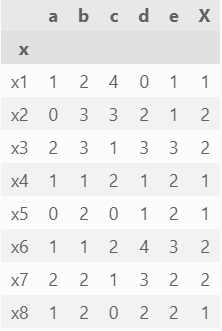
\includegraphics[scale=0.8]{img/df_exemple_3.PNG}
	\caption{Dataframe "df3"}
	\label{fig:df_exemple_3}
\end{figure}
Appliquons étapes par étapes l'algorithme \quickreduct.\\
Nous commençons avec $R = \emptyset $.\\
Puis nous calculons la dépendance pour chaque attributs :\\
$\gamma_{\{a\}}(X) = 2/8$ \\
$\gamma_{\{b\}}(X) = 2/8$ \\
$\gamma_{\{c\}}(X) = 6/8$ \\
$\gamma_{\{d\}}(X) = 6/8$ \\
$\gamma_{\{e\}}(X) = 2/8$ \\
Nous ajoutons l'attribut possèdant la plus haute dépendance, ici $\{c\}$. \\
Nous changéons la valeur de R, $R = \{c\}$. \\
Nous re-calculons la dépendance en faisant des combinaisons avec $\{c\}$. \\
$\gamma_{\{\textcolor{red}{c},a\}}(X) = 6/8$ \\
$\gamma_{\{\textcolor{red}{c},b\}}(X) = 6/8$ \\
$\gamma_{\{\textcolor{red}{c},d\}}(X) = 8/8$ \\
Nous obtenons la même dépendance qu'avec tous les attrbiuts, nous pouvons
arrêter de calculer, nous avons trouvé la réduction. \\
$R = \{\textcolor{red}{c}, \textcolor{blue}{d}\}$ \\
Avec notre algorithme nous avons :
\begin{lstlisting}
R3 = quickReduct(df3, "X")
Python> C : ['a', 'b', 'c', 'd', 'e']
dep_C : 1
lambda([]) = 0
lambda(['a']) = 1/4
changement R = ['a']
lambda(['b']) = 1/4
lambda(['c']) = 3/4
changement R = ['c']
lambda(['d']) = 3/4
lambda(['e']) = 1/4
lambda(['c']) = 3/4
lambda(['c']) = 3/4
lambda(['c', 'a']) = 3/4
lambda(['c', 'b']) = 3/4
lambda(['c', 'd']) = 1
changement R = ['c', 'd']
lambda(['c', 'e']) = 1
lambda(['c', 'd']) = 1
Réduction =  ['c', 'd']
\end{lstlisting}